\documentclass[]{article}

\usepackage{tkz-base}
\usepackage{tikz}
\usepackage{amsmath}
\usepackage{amsfonts}
\usepackage{amssymb}
\usepackage{tkz-euclide}

\usetikzlibrary{svg.path}
\usetikzlibrary{snakes}
\usetikzlibrary{arrows}

%opening
\title{Jacobians -- Velocity Transformation}
\author{Craig Carignan\\Glen Henshaw}

\begin{document}

\maketitle

\begin{abstract}

\end{abstract}

Jacobian (Ref Sec. 5.7; Exercises 5.17, SS 3.1, SS 3.2)

\subsection{Jacobians}
The ``Jacobian'' is actually a ``Jacobian matrix'' which relates the differentials of one coordinate set to another:

\begin{eqnarray}
y_{1} & = & f_{1}(x_{1}, x_{2}) \\
y_{2} & = & f_{2}(x_{1}, x_{2}) \\
\textrm{or}\nonumber \\ 
\underline{y} & = & \underline{f}(\underline{x}) 
\end{eqnarray}
Taking partial derivatives of both sides, we get
\begin{displaymath}
	\delta \underline{y} = \frac{\partial \underline{f}}{\partial \underline{x}}\delta\underline{x}
\end{displaymath}
\begin{displaymath}
\frac{\partial \underline{f}}{\partial \underline{x}} = \left[
	\begin{array}{cc}
		\frac{\partial f_{1}}{\partial x_{1}} & \frac{\partial f_{1}}{\partial x_{2}} \\
		\frac{\partial f_{2}}{\partial x_{1}} & \frac{\partial f_{2}}{\partial x_{2}} \\
	\end{array}
	\right]
\end{displaymath}
or
\begin{equation}
	\dot{\underline{y}} = \frac{\partial \underline{f}}{\partial \underline{x}} \dot{\underline{x}} \equiv J\dot{\underline{x}}
\end{equation}
Note that $J \equiv J(\underline{x})$ if $\underline{f}(\underline{x})$ is nonlinear.

In robotics, the two coordinate sets are typically the joint angles and the end effector pose (position and orientation):
\begin{equation}
	\underbrace{\left[ \begin{array}{c} ^{i}\underline{\mathcal{V}} \\ ^{i}\underline{\omega} \end{array}\right]}_{\substack{\text{tool} \\ \text{velocity} \\ [M]}} = \underbrace{\left[ \begin{array}{c} ^{i}J_{tran} \\ ^{i}J_{rot} \end{array} \right]}_{\substack{\textrm{Jacobian}\\ J \\ [M \times N]}} \underbrace{\dot{\underline{q}}}_{\substack{\textrm{joint}\\ \text{rates}\\ [N]}} 
\end{equation}
where
\begin{displaymath}
	\dot{\underline{q}}_{i} = \left\{
	\begin{array}{cl} \dot{\underline{\theta}}_{i} & \textrm{revolute} \\
	\dot{\underline{d}}_{i} & \textrm{prismatic} \end{array}
	\right.
\end{displaymath}
So the Jacobian $J$ transforms vectors of joint rates to vectors of end effector rates:
\\
\\

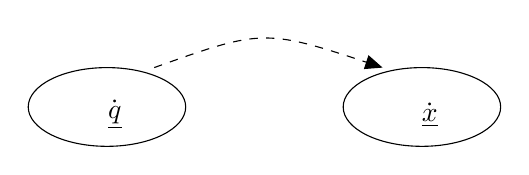
\begin{tikzpicture}
	\draw[snake=expanding waves,segment angle=7] (0,0) ellipse (1cm and 0.5cm);
	\draw (4,0) ellipse (1cm and 0.5cm);
	\draw (0.1, -0.1) node{$\dot{\underline{q}}$};
	\draw (4.1, -0.1) node{$\dot{\underline{x}}$};
	\draw[dashed][arrows=-triangle 45] (0.6, 0.5) .. controls (2, 1) .. (3.5, 0.5);
\end{tikzpicture}
\\
\\
 
\subsection{EXAMPLE: Polar robot translation Jacobian}

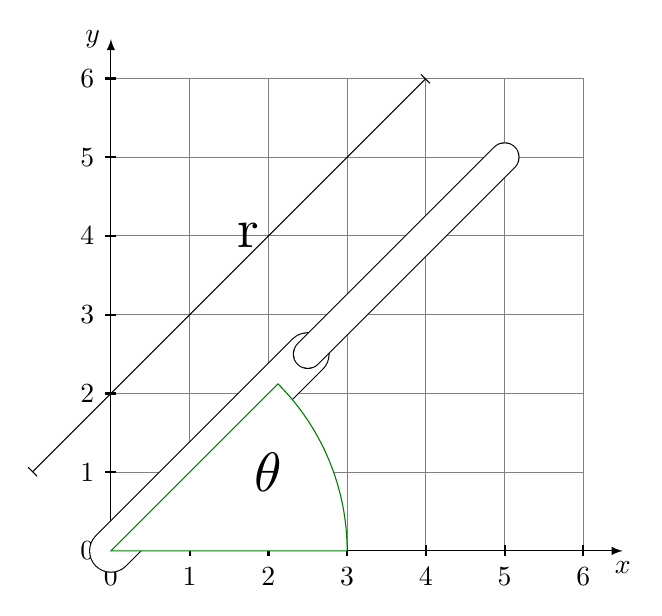
\begin{tikzpicture}
	\tkzInit[xmax=6,ymax=6,xmin=0,ymin=0]
	\tkzGrid
	\tkzAxeXY
	\draw[double=none, double distance=15pt, line join=round, line cap=round] (0.0, 0.0) -- (2.5, 2.5);
	\draw[double=none, double distance=10pt, line join=round, line cap=round] (2.5, 2.5) -- (5.0, 5.0);
	\draw[arrows=|-|] (-1, 1) -- (4.0, 6);
	\draw (1.75, 4.0) node[label={[scale=2]center:r}]{};
	\filldraw[fill=white, draw=green!50!black] (0,0) -- (30mm,0mm) arc (0:45:30mm) -- cycle;
	\draw (2,1) node[label={[scale=2]center:$\theta$}]{};
\end{tikzpicture}

Let's first write the forward kinematics for this arm. From inspection,
\begin{eqnarray}
x & = & r \cos \theta \nonumber \\
y & = & r \sin \theta \nonumber
\end{eqnarray}
or
\begin{displaymath}
	\underbrace{\left[ \begin{array}{c} x \\ y \end{array} \right]}_{\underline{p}} = \underbrace{\left[ \begin{array}{c} r \cos \theta \\ r \sin \theta \end{array} \right]}_{\underline{f}(r, \theta)}
\end{displaymath}
or
\begin{displaymath}
	\underline{p} = \underline{f}(\underline{q})
\end{displaymath}
where
\begin{eqnarray}
\underline{p} & = & [x\ \ y]^{t} \nonumber \\
\underline{q} & = & [r\ \ \theta]^{t} \nonumber
\end{eqnarray}
then
\begin{equation}
	\dot{\underline{p}} = J_{tran}(\underline{q}) \Rightarrow J_{tran}(\underline{q}) \left[ \begin{array}{cc} \frac{\partial x}{\partial r} & \frac{\partial x}{\partial \theta} \\ \frac{\partial y}{\partial r} & \frac{\partial y}{\partial \theta} \end{array} \right] = \left[ \begin{array}{cc} \cos \theta & -r \sin \theta \\ \sin \theta & r \cos \theta \end{array} \right]
\end{equation}
This is the ``direct differentiation'' method. Works okay for arms with few degrees of freedom. Completely intractable for most arms.

Okay, what about rotation?
\begin{displaymath}
	\Omega = \dot{R}(\underline{q})R(\underline{q})^{T}
\end{displaymath}
where
\begin{displaymath}
\Omega \triangleq \left[ \begin{array}{ccc} 0 & -\omega_{z} & \omega_{y} \\
\omega_{z} & 0 & -\omega_{x} \\ -\omega_{y} & \omega_{x} & 0 \end{array} \right]
\end{displaymath}
and
\begin{displaymath}
\underline{\omega} = \left[ \begin{array}{c} \omega_{x} \\ \omega_{y} \\ \omega_{x} \end{array} \right].
\end{displaymath}
\\

\begin{displaymath}
\dot{R} = \sum_{j=1}^{N} \frac{\partial R(\underline{q})}{\partial q_{j}}\dot{q}_{j}
\end{displaymath}
can be rewritten as
\begin{displaymath}
	\underline{\omega}=J_{rot}\dot{\underline{q}}
\end{displaymath}
See Exercise 5.16. and the RPR Wrist Jacobian handout.

This is the ``Direct Differentiation'' method for the rotation Jacobian, and it is very tedious.

\subsection{Cross--product method}
There is an alternative method called the ``cross--product method'' which is more computationally efficient and derives from the velocity propagation method. It's based on the insight that each element of the Jacobian describes the instantaneous motion of the end effector along some direction in terms of the motion of each joint. Graphically:

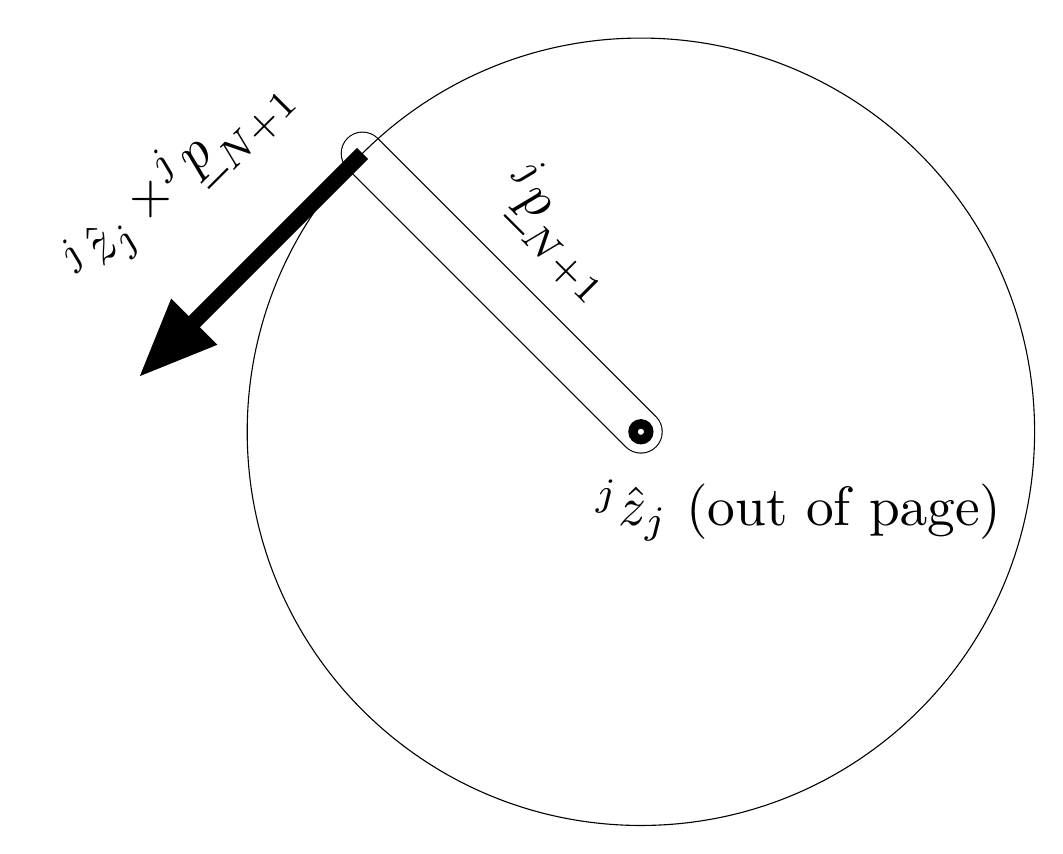
\begin{tikzpicture}
	\draw[double=none, double distance=15pt, line join=round, line cap=round] (0,0) -- (-5*0.707, 5*0.707) node[label={[yshift=-1cm, xshift=2.5cm, rotate=-45, scale=2]center:$^{j}\underline{p}_{N+1}$}]{};
	\draw[line width=1.2mm] (0,0) circle (1mm);
	\draw (0,0) circle (5cm) node[xshift=2.0cm, yshift=-1.0cm, label={[scale=2]center:$^{j}\hat{z}_{j}$ (out of page)}]{};
	\draw[line width=2mm][arrows=-triangle 45] (-5*0.707, 5*0.707) -- (-5*0.707-4*0.707, 5*0.707-4*0.707) node[label={[yshift=2.5cm, xshift=0.5cm, rotate=45, scale=2]center:$^{j}\hat{z}_{j} \times^{j}\!\underline{p}_{N+1}$}]{};
\end{tikzpicture}
\\
\\

where the circle is the set of points swept out by the end effector and the solid arrow shows the current velocity of the end effector, which of course is normal to the circle. Finding the direction of this vector is, of course, a simple matter of crossing the unit vector passing through the link's center of rotation (out of the plane of the page) with the vector from the center of rotation to the end effector.

Formally, let
\begin{displaymath}
	^{i}\hat{z}_{j} \triangleq\ ^{i}(^{j}\hat{z}_{j})
\end{displaymath}
i.e. the third column of $^{i}_{j}R =\ ^{i}_{j}R\ ^{j}z_{j}$. Then,
\begin{displaymath}
^{i}J_{rot} = \left[\ ^{i}\hat{z}_{1}, ^{i}\hat{z}_{2}, \cdots, ^{i}\hat{z}_{N}\right] \Lambda
\end{displaymath}
where
\begin{displaymath}
	\Lambda \triangleq \text{diag}(\lambda_{i})\ \text{with}\ \lambda_{i} = \left\{ \begin{array}{cl} 1 & \text{revolute} \\ 0 & \text{prismatic} \end{array} \right.
\end{displaymath}
and
\begin{displaymath}
\begin{split}
^{i}J_{trans} & = \left[\ \!^{i}\hat{z}_{1} \times\ ^{i}(\ \! ^{1}\underline{p}_{N+1}), \ \!^{i}\hat{z}_{2} \times\ ^{i}(\ \! ^{2}\underline{p}_{N+1}), \ \!^{i}\hat{z}_{3} \times\ ^{i}(\ \! ^{3}\underline{p}_{N+1})\right] \Lambda \\
& + (I_{N \times N} - \Lambda) \left[\ \!^{i}\hat{z}_{1}, \ \!^{i}\hat{z}_{2}, \cdots, \ \!^{i}\hat{z}_{N} \right]
\end{split}
\end{displaymath}

\subsection{Changing the frame of the Jacobian}
Given $^{B}J$, find $^{A}J$.

By definition,
\begin{displaymath}
\left[\begin{array}{c} ^{B}\underline{\mathcal{V}}_{p} \\ ^{B}\underline{\omega} \end{array} \right] = ^{B}J(\underline{q})\underline{\dot{q}}
\end{displaymath}
Velocity is a free vector, so:
\begin{displaymath}
\left. \begin{array}{ccl} ^{A}\underline{\mathcal{V}}_{p} & = & ^{A}_{B}R\ \!^{B}\underline{\mathcal{V}}_{p} \\ ^{A}\underline{\omega} & = & ^{A}_{B}R\ \!^{B}\underline{\omega} \end{array} \right\} \Rightarrow \left[\begin{array}{c} ^{A}\underline{\mathcal{V}}_{p} \\ ^{A}\underline{\omega} \end{array} \right] = \left[ \begin{array}{cc} \ \!^{A}_{B}R & 0_{3 \times 3} \\ 0_{3 \times 3} &  \ \!^{A}_{B}R \end{array} \right]^{B}J(\underline{q})\dot{\underline{q}})
\end{displaymath}

\subsection{Example: 3--link planar manipulator}
\begin{figure}
	\centering
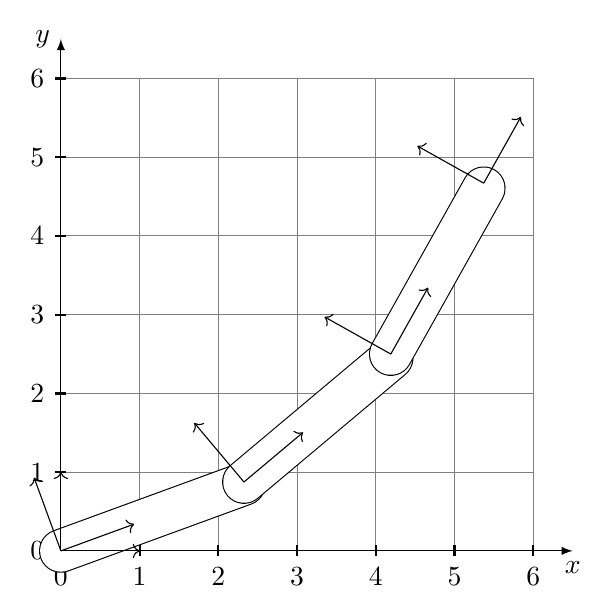
\begin{tikzpicture}
\tkzInit[xmax=6,ymax=6,xmin=0,ymin=0]
\tkzGrid
\tkzAxeXY
\draw[cm={0.93,0.34,-0.34,0.93,(0,0)}][double=none, double distance=15pt, line join=round, line cap=round] (0.0, 0.0) -- (2.5, 0);
\draw[cm={0.93,0.34,-0.34,0.93,(0, 0)}][->] (0.0, 0.0) -- (1.0, 0.0);
\draw[cm={0.93,0.34,-0.34,0.93,(0, 0)}][->] (0.0, 0.0) -- (0.0, 1.0);

\draw[cm={0.75,0.63,-0.63,0.75,(2.325, 0.875)}][double=none, double distance=15pt, line join=round, line cap=round] (0.0, 0.0) -- (2.5, 0);
\draw[cm={0.75,0.63,-0.63,0.75,(2.325, 0.875)}][->] (0.0, 0.0) -- (1.0, 0.0);
\draw[cm={0.75,0.63,-0.63,0.75,(2.325, 0.875)}][->] (0.0, 0.0) -- (0.0, 1.0);

\draw[cm={0.472,0.842,-0.842,0.472,(4.19, 2.5)}][double=none, double distance=15pt, line join=round, line cap=round] (0.0, 0.0) -- (2.5, 0);
\draw[cm={0.472,0.842,-0.842,0.472,(4.19, 2.5)}][->] (0.0, 0.0) -- (1.0, 0.0);
\draw[cm={0.472,0.842,-0.842,0.472,(4.19, 2.5)}][->] (0.0, 0.0) -- (0.0, 1.0);

\draw[->] (0.0, 0.0) -- (1.0, 0.0);
\draw[->] (0.0, 0.0) -- (0.0, 1.0);

\draw[cm={0.472,0.842,-0.842,0.472,(5.37, 4.67)}][->] (0.0, 0.0) -- (1.0, 0.0);
\draw[cm={0.472,0.842,-0.842,0.472,(5.37, 4.67)}][->] (0.0, 0.0) -- (0.0, 1.0);
\end{tikzpicture}
\end{figure}

\subsubsection{A: Find $^{i}J_{rot} \Rightarrow\ \!^{0}_{1}R\ \!^{1}_{2}R$ }
\begin{displaymath}
^{0}_{1}R = \left[ \begin{array}{ccc} c_{1} & -s_{1} & 0 \\ s_{1} & c_{1} & 0 \\ 0 & 0 & 1 \end{array} \right],\ \ ^{0}_{2}R = \left[ \begin{array}{ccc} c_{12} & -s_{12} & 0 \\ s_{12} & c_{12} & 0 \\ 0 & 0 & 1 \end{array} \right],\ \ ^{0}_{3}R = \left[ \begin{array}{ccc} c_{123} & -s_{123} & 0 \\ s_{123} & c_{123} & 0 \\ 0 & 0 & 1 \end{array} \right]
\end{displaymath}
\begin{displaymath}
^{0}J_{rot} = \left[ \begin{array}{ccc} 0 & 0 & 0 \\ 0 & 0 & 0 \\ 1 & 1 & 1 \end{array}\right] = \ \! ^{2}J_{rot} \Rightarrow \ \!^{0}\underline{\omega}_{3} = \ \! ^{2}\underline{\omega}_{3} = \left[ \begin{array}{c} 0 \\ 0 \\ \dot{\theta}_{1}+\dot{\theta}_{2}+\dot{\theta}_{3} \end{array} \right]
\end{displaymath}
\subsubsection{B: Find $\ \!^{i}J_{trans}$}
(1) Use differentiation method
\begin{displaymath}
^{0}\underline{p}_{4} = \left[ \begin{array}{c} l_{1}c_{1} + l_{2}c_{12} + l_{3}c_{123} \\ l_{1}s_{1} + l_{2}s_{12} + l_{3}s_{123} \\ 0 \end{array} \right]
\end{displaymath}
Factoring,
\begin{displaymath}
^{0}j_{trans} = \frac{\partial \ \!^{0}\underline{p}_{4}}{\partial \underline{\theta}} = \left[\begin{array}{ccc} -l_{1}s_{1}-l_{2}s_{12}-l_{3}s_{123} & -l_{2}s_{12}-l_{3}s_{123} & -l_{3}s_{123} \\ l_{1}c_{1} +l_{2}c_{12} +l_{3}c_{123} & l_{2}c_{12} + l_{3}c_{123} & l_{3}c_{123} \\ 0 & 0 & 0 \end{array}\right]
\end{displaymath}
\begin{displaymath}
	^{2}J_{tran} = \ \!^{2}_{0}R\ \!^{0}J = \left[\begin{array}{ccc} c_{12} & s_{12} & 0 \\ -s_{12} & c_{12} & 0 \\ 0 & 0 & 1 \end{array} \right] \left[\begin{array}{ccc} -l_{1}s_{1}-l_{2}s_{12}-l_{3}s_{123} & -l_{2}s_{12}-l_{3}s_{123} & -l_{3}s_{123} \\ l_{1}c_{1} +l_{2}c_{12} +l_{3}c_{123} & l_{2}c_{12} + l_{3}c_{123} & l_{3}c_{123} \\ 0 & 0 & 0 \end{array}\right]
\end{displaymath}
or
\begin{displaymath}
= \left[ \begin{array}{ccc} l_{1}s_{2} - l_{3}s_{3} & -l_{3}s_{3} & -l_{3}s_{3} \\ l_{1}c_{2}+l_{2} + l_{3}c_{3} & l_{2}+l_{3}c_{3} & l_{3}c_{3} \\ 0 & 0 & 0 \end{array} \right]
\end{displaymath}
Notice that $^{2}J_{tran}$ is much simpler than $^{0}J_{tran}$.

(2) Use ``Cross Product'' method

\begin{displaymath}
^{0}J_{tran} = \left[ \begin{array}{ccc} \ \!^{0}\hat{z}_{1} \times \ \!^{0}(\ \!^{1}\underline{p}_{4}) & \ \!^{0}\hat{z}_{2} \times \ \!^{0}(\ \!^{2}\underline{p}_{4}) & \ \!^{0}\hat{z}_{3} \times \ \!^{0}(\ \!^{3}\underline{p}_{4}) \end{array} \right]
\end{displaymath}
\begin{displaymath}
^{0}\hat{z}_{1} = \ \!^{0}\hat{z}_{2} = \ \!^{0}\hat{z}_{3} = \left[\begin{array}{c} 0 \\ 0 \\ 1 \end{array}\right]
\end{displaymath}
\begin{displaymath}
^{3}\underline{p}_{4} = \left[ \begin{array}{c} l_{3} \\ 0 \\ 0 \end{array}\right]
\end{displaymath}
\begin{displaymath}
^{2}\underline{p}_{3} = \left[ \begin{array}{c} l_{2} \\ 0 \\ 0 \end{array}\right]
\end{displaymath}
\begin{displaymath}
^{1}\underline{p}_{2} = \left[ \begin{array}{c} l_{1} \\ 0 \\ 0 \end{array}\right]
\end{displaymath}
so
\begin{displaymath}
^{0}(^{3}\underline{p}_{4}) = \left[ \begin{array}{c} l_{3}c_{123} \\ l_{3}s_{123} \\ 0 \end{array} \right]
\end{displaymath}

\begin{displaymath}
^{0}(\ \!^{2}\underline{p}_{4}) = \ \!^{0}(\ \!^{2}\underline{p}_{3}) + \ \!^{0}(\ \!^{3}\underline{p}_{4}) = \left[ \begin{array}{c} l_{2}c_{12}+l_{3}c_{123} \\ l_{2}s_{12} + l_{3}s_{123} \\ 0 \end{array} \right]
\end{displaymath}
\begin{displaymath}
^{0}(\ \!^{1}\underline{p}_{4}) = \ \!^{0}(\ \!^{1}\underline{p}_{2}) + \ \!^{0}(\ \!^{2}\underline{p}_{4}) = \left[ \begin{array}{c} l_{1}c_{1}+l_{2}c_{12}+l_{3}c_{123} \\ l_{1}s_{1} + l_{2}s_{12} + l_{3}s_{123} \\ 0 \end{array} \right]
\end{displaymath}
Note that these two equations can be obtained recursively. Performing the cross product yields the same result for $^{0}J_{trans}$:

\begin{displaymath}
	\left[\begin{array}{c} 0 \\ 0 \\ 1 \end{array}\right] \times ^{0}(\ \!^{1}\underline{p}_{4}) =\left[ \begin{array}{c} -l_{1}s_{1}-l_{2}s_{12}-l_{3}s_{123} \\ l_{1}c_{1} + l_{2}c_{12} + l_{3}c_{123} \\ 0 \end{array}\right]
\end{displaymath}

\begin{displaymath}
	\left[\begin{array}{c} 0 \\ 0 \\ 1 \end{array}\right] \times ^{0}(\ \!^{2}\underline{p}_{4}) =\left[ \begin{array}{c} -l_{2}s_{12}-l_{3}s_{123} \\  l_{2}c_{12} + l_{3}c_{123} \\ 0 \end{array}\right]
\end{displaymath}

and

\begin{displaymath}
	\left[\begin{array}{c} 0 \\ 0 \\ 1 \end{array}\right] \times ^{0}(\ \!^{3}\underline{p}_{4}) = \left[ \begin{array}{c} -l_{3}s_{123} \\ l_{3}c_{123} \\ 0 \end{array}\right]
\end{displaymath}

Assembling these vectors into the Jacobian matrix gives the same result as with the direct differentiation method:

\begin{displaymath}
^{0}j_{trans} = \left[\begin{array}{ccc} -l_{1}s_{1}-l_{2}s_{12}-l_{3}s_{123} & -l_{2}s_{12}-l_{3}s_{123} & -l_{3}s_{123} \\ l_{1}c_{1} +l_{2}c_{12} +l_{3}c_{123} & l_{2}c_{12} + l_{3}c_{123} & l_{3}c_{123} \\ 0 & 0 & 0 \end{array}\right]
\end{displaymath}

To compute $^{2}J_{trans}$, we do the same calculations, but in frame 2:

\begin{displaymath}
^{2}J_{trans} = \left[ \begin{array}{ccc} \ \!^{2}\hat{z}_{1} \times \ \!^{2}(\ \!^{1}\underline{p}_{4}) & \ \!^{2}\hat{z}_{2} \times \ \!^{2}(\ \!^{2}\underline{p}_{4}) & \ \!^{2}\hat{z}_{3} \times \ \!^{2}(\ \!^{3}\underline{p}_{4})\end{array}\right]
\end{displaymath}
In our example, $^{2}\hat{z}_{1} = \ \!^{2}\hat{z}_{2} = ^{2}\hat{z}_{3} = [0\ 0\ 1]^{T}$, so starting with the last term:
\begin{displaymath}
^{2}(\ \!^{3}\underline{p}_{4}) = \left[ \begin{array}{c} l_{3}c_{3} \\ l_{3}s_{3} \\ 0 \end{array}\right]
\end{displaymath}
then
\begin{displaymath}
^{2}(\ \!^{2}\underline{p}_{4}) = \ \!^{2}(\ \!^{2}\underline{p}_{3}) + \ \!^{2}(\ \!^{3}\underline{p}_{4}) = \left[ \begin{array}{c} l_{2} \\ 0 \\ 0 \end{array} \right] + \left[ \begin{array}{c} l_{3}c_{3} \\ l_{3}s_{3} \\ 0 \end{array}\right]
\end{displaymath}
and finally
\begin{displaymath}
^{2}(\ \!^{1}\underline{p}_{4}) = \left[\begin{array}{ccc}c_{2} & s_{2} & 0 \\ -s_{2} & c_{2} & 0 \\ 0 & 0 & 1 \end{array}\right]\left[\begin{array}{c} l_{1} \\ 0 \\ 0 \end{array}\right] + \left[\begin{array}{c} l_{2} + l_{3}c_{3} \\ l_{3}s_{3} \\ 0 \end{array} \right] = \left[\begin{array}{c} l_{2}+l_{2}c_{2}+l_{3}c_{3} \\ -l_{2}s_{2} + l_{3}s_{3} \\ 0 \end{array}\right]
\end{displaymath}
Performing the cross product yields the same results for $^{2}J_{trans}$. Notice how much easier it is to compute using this method!
\end{document}


